\documentclass[10pt,a4paper]{article}

\usepackage[utf8]{inputenc}


\usepackage{algpseudocode}
\usepackage{algorithmicx}
\usepackage{amsfonts}
\usepackage{amsmath}
\usepackage{amssymb}
\usepackage[spanish]{babel}
\usepackage[style=nature,intitle=true,sorting=none]{biblatex}
\usepackage{csquotes}
\usepackage{dsfont}
\usepackage{enumitem}
\usepackage{fancyhdr}
\usepackage{geometry}
\usepackage{graphicx}
\usepackage[hidelinks]{hyperref}
\usepackage{ifthen}
\usepackage[utf8]{inputenc}
\usepackage{multicol}
\usepackage{titling}
\usepackage{xcolor}
\usepackage{wrapfig}


\title{Organización del Computador I}
\author{Gianfranco Zamboni}

%%%% CONFIGURACIONES %%%%

%% La coma de los reales es un punto
\decimalpoint

%%% Tamaño de pagina
%\geometry{
%	includeheadfoot,
%	left=2.54cm,
%	bottom=1cm,
%	top=1cm,
%	right=2.54cm
%}

%\stul{0.1cm}{0.2ex}

%% HEADER Y FOOTER
\pagestyle{fancy}

\fancyhf{}

\fancyhead[LO]{\rightmark} % \thesection\ 
\fancyhead[RO]{\small{\thetitle}}
\fancyfoot[CO]{\thepage}
\renewcommand{\headrulewidth}{0.5pt}
\renewcommand{\footrulewidth}{0.5pt}
\setlength{\headsep}{1cm}
\setlength{\headheight}{13.07225pt}

\renewcommand{\baselinestretch}{1.2}  % line spacing

%% Links en indice 
\hypersetup{
	linktoc=all,     %set to all if you want both sections and subsections linked
	linkcolor=blue,  %choose some color if you want links to stand out
}

\newcommand{\red}[1]{{\color{red}#1}}  			% Rojo, duh (?)
\begin{document}
	\maketitle
	\tableofcontents
	\newpage

\section{Arquitectura de Von Neumann}
El siguiente diagrama muestra como está conformada una computadora básica que usa este tipo de sistemas:

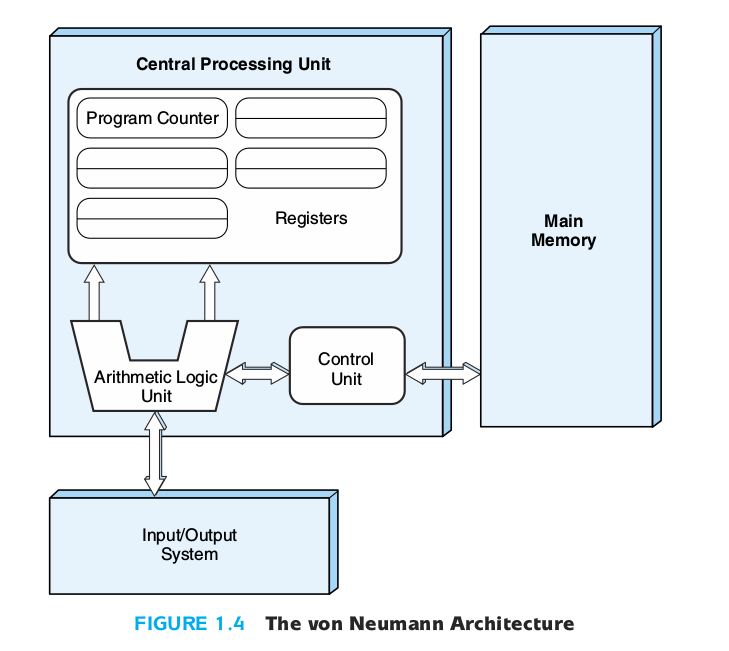
\includegraphics[width=15cm, keepaspectratio=yes]{imagenes/von_neumann.png}

Se puede ver que consta de 3 componentes principales:
\begin{itemize}
	\item Una \textbf{memoria principal} (main memory) en donde se guardan los programas (secuencia de instrucciones) que controlan las operaciones realizadas por la computadora.
	\item Un \textbf{sistema de entrada/salida}
	\item Una \textbf{unidad central de procesamiento} (Central Processing Unit, CPU) que contiene una \textbf{ALU} (Arithmetic Logic Unit) para realizar operaciones aritméticas y lógicas, una \textbf{unidad de control} (Control Unit, CU) que comunica la ALU con la memoria principal y un conjunto de registros entre los cuales se encuentra el \textbf{Program Counter} (PC) que indica donde se encuentra la próxima instrucción que debe ser ejecutada.
\end{itemize}

Este tipo de arquitectura es capaz de llevar a cabo el procesamiento de instrucciones de manera secuencial y uno de sus grandes problemas, conocido como \textit{cuello de botella de Von Neumann}, es que no puede realizar operaciones de datos y una extracción de instrucción simultanea debido a que la unidad de control y la memoria principal están conectados por un único camino que solo permite usar dichos componentes para una extracción de instrucción o para una operación de datos, pero no ambas a la vez.

\subsection{Ciclo de ejecución de Von Neumman}
\begin{center}
	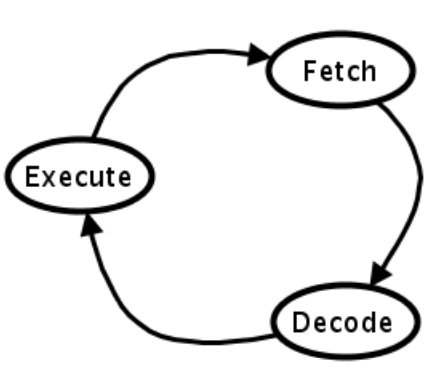
\includegraphics[width=5cm, keepaspectratio=yes]{imagenes/von_neumann_cycle.png}
\end{center}
Arriba, se muestra el ciclo de ejecución de Von Neumann, una iteración de dicho ciclo está caracterizada por 3 etapas:
\begin{itemize}
	\item \textbf{Fetch}: La unidad de control busca, en memoria, la próxima instrucción a ser ejecutada usando la información del program counter.
	\item \textbf{Decode}: La unidad de control decodifica la instrucción para que sea entendible por la ALU y, si es necesario, busca en la memoria los datos necesitados para la correcta ejecución de la misma.
	\item \textbf{Execute}: La ALU ejecuta la instrucción decodificada y guarda los resultados en los registros o en la memoria.
\end{itemize}

\newpage

\section{Entrada/Salida}
Se define un subsistema de I/O como un conjunto de componente que mueven datos entre dispositivos externos y un host compuesto por una CPU y un memoria principal.

\begin{center}
	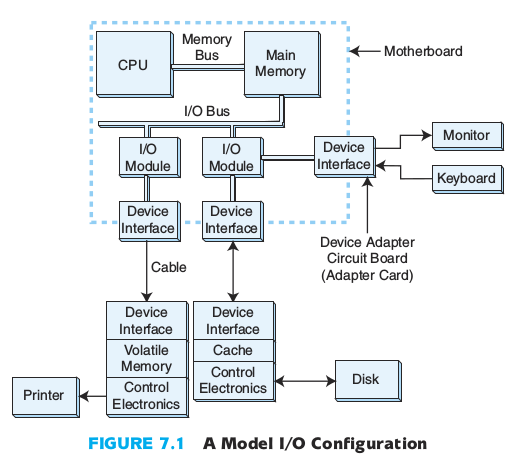
\includegraphics[width=15cm, keepaspectratio=yes]{imagenes/iomodel.png}
\end{center}

Por lo general, un sistema de I/O esta compuesto por:
\begin{itemize}
	\item Bloques de memoria principal dedicadas a funciones de entrada/salida
	\item Buses por los que se mueven distintos tipos de datos desde la memoria hacia los dispositivos y viceversa.
	\item Modulos de control, tanto en el host, como en los dispositivos que aseguran la correcta ejecución de las tareas de I/O.
	\item Modulos I/O que indican hacia dónde y desde dónde debe llegar la información.
\end{itemize}

Además, se necesita un mecanismo para controlar el funcionamiento de los distintos dispositivos y prevenir, de esta forma, los problemas que podría ocasionar, por ejemplo, la escritura en memoria de dos o más de ellos a la vez.

\subsection{Polling}
Se asigna un registro de usa exclusivo a cada dispositivo. La CPU monitorea constantemente cada uno de estos registros esperando a que algunos de los dispositivos escriba en su registro el estado \textit{data ready} indicando, de esta manera, que desea realizar una operación de entrada/salida.

Uno de las grandes desventajas de este método es que, mientras no haya ningún request para hacer operaciones de I/O, la CPU se mantiene en el loop constante descripto mas arriba, prohibiéndole realizar cualquier otro tipo de tareas.

\subsection{Interrupciones}
Se agrega, al registro de flags del CPU, un flag de interrupción que indica cuando un dispositivo necesita realizar una operación de I/O. Por lo general para implementar un sistemas con interrupciones se usa un controlador de interrupciones (IC):

\begin{center}
	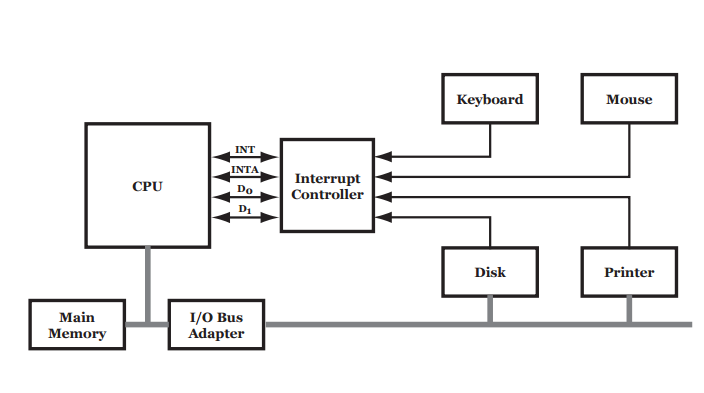
\includegraphics[width=12cm, keepaspectratio=yes]{imagenes/iointerruptio.png}
\end{center}

Los dispositivos se conectan al IC y cuando necesitan realizar alguna operación mandan una señal al mismo. Este, recibe la señal y manda la señal INT al CPU, activando su flag de interrupciones. El CPU termina de ejecutar la instrucción en curso y verifica si hay interrupciones pendientes. Si las hay, notifica al IC con la señal INTA indicando que está lista para atender el request y, entonces, el IC le envía el id del dispositivo que pidió el request.

Una vez hecho esto, el CPU guarda el contexto del programa que se está ejecutando, deshabilita las interrupciones y ejecuta la rutina de atención de interrupciones correspondientes. Por último, la CPU restaura el contexto del programa, vuelve a habilitar las interrupciones y vuelve a ejecutar el programa desde donde lo habia dejado.

\subsection{Direct Memory Access (DMA)}
Para mejorar el rendimiento del CPU durante las operaciones de I/O que implican transferencia de datos entre la memoria principal y algún dispositivo particular, se agrega un DMA Controller. Cuando este dispositivo se encuentra presente y se debe realizar una operación de este tipo, el CPU envia al DMA donde se encuentran los bytes que deben ser copiados, la cantidad que debe copiar y a dónde deben ser copiados.

\begin{center}
	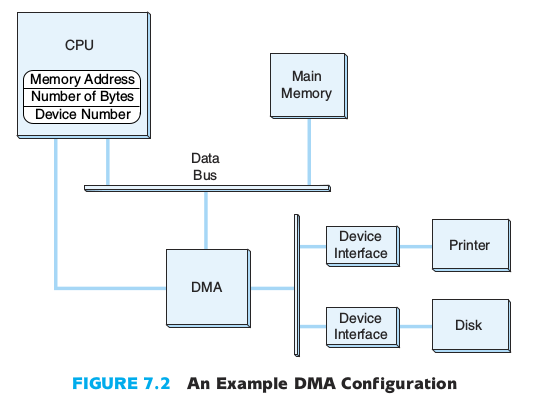
\includegraphics[width=12cm, keepaspectratio=yes]{imagenes/iodma.png}
\end{center}

Una vez que la transferencia es completada, el DMA manda una señal de interrupción al CPU indicando la finalización de la misma. 

Se puede ver que el DMA y el CPU comparten el mismo bus de memoria, por lo que sólo uno de ellos puede realizar operaciones de lectura/escritura sobre la memoria principal. Por lo general, las operaciones de I/O tienen mayor prioridad que las del CPU debido a que una larga espera inactiva del dispositivo podría llevar a un timeout implicando la cancelación de la operación.

\subsection{I/O Bus}
Además del DMA, se puede resolver el problema del bus agregando buses dedicados. Es decir un bus para datos, otro para direcciones y otro de control:

\begin{center}
	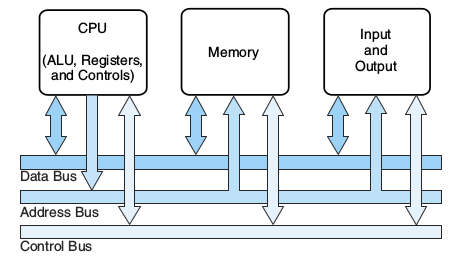
\includegraphics[width=10cm, keepaspectratio=yes]{imagenes/iobuses.png}
\end{center}

\begin{center}
	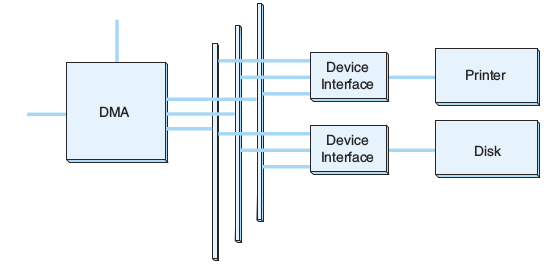
\includegraphics[width=10cm, keepaspectratio=yes]{imagenes/dmabus.png}
\end{center}

El bus de control es necesario para enviar y recibir señales que indiquen el status de los dispositivos que intervienen en la comunicación, ya que se debe tomar en cuenta que estos funcionan a distintas velocidades y no es posible realizar operaciones sincrónicas (que dependan de un único reloj compartido para todos los dispositivos).

\subsection{Cuadro comparativo}
\begin{center}
	\begin{center}
		\begin{tabular}{|c|c|c|c|}
			\hline
			Método I/O & Complejidad hardware & Complejidad software & Velocidad\\ 
			\hline \hline 
			Polling &  $+$  & $+++$ & $+$ \\
			Interrupciones &  $++$  & $++$ & $++$ \\
			DMA &  $+++$  & $+$ & $+++$ \\
			\hline
		\end{tabular}
	\end{center}
\end{center}

\subsection{Channel I/O}
Los métodos vistos hasta el momento transfieren data de a bytes o en pequeños bloques y en el caso de falla se le comunica a la CPU, la cual debe determinar los pasos a realizar a continuación. Estos funcionan bien en sistemas pequeños pero no escalan bien a grandes sistemas multiusuarios. Para estos casos se suele usar una configuración \textbf{Channel I/O}.

\begin{center}
	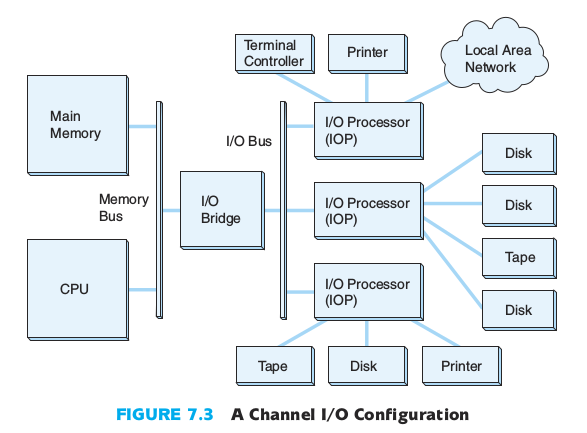
\includegraphics[width=15cm, keepaspectratio=yes]{imagenes/iochannel.png}
\end{center}

Cada canal de I/O es controlado por un \textbf{I/O Processor (IOP)} que ejecutan programas especificos de transferencia de datos y contienen distintos comandos de control especializados para los dispositivos conectados.

En este método, cuando una operación es requerida el IOP manda un señal de interrupción a la CPU. El CPU busca el programa que dicho IOP debe ejecutar y le envia la dirección en la que debe empezar a ejecutar. El IOP ejecuta la rutina de atención y finalmente manda una nueva interrupción a la CPU para indicar que finalizó su tarea.

\newpage

\newpage

\section{Buses}
Un bus es un camino de comunicación entre dos o mas dispositivos. Una característica clave es que se trata de un medio de transmisión compartido. Si dos o más dispositivos transmiten durante el mismo período de tiempo, sus señales puedes solaparse y distorsionarse.

\begin{center}
	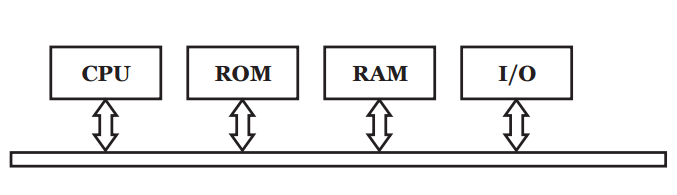
\includegraphics[width=10cm, keepaspectratio=yes]{imagenes/bus.png}
\end{center}

Las computadoras poseen diferentes tipos de buses que proporcionan comunicación entre sus componentes dentro de la jerarquía del sistema. El bus que conecta los componentes principales del computador se denomina \textbf{Bus del sistema}. Dicho bus está compuesto por entre 50 y 100 líneas que pueden ser clasificadas en 3 tipos: líneas de datos, de direcciones y de control.

\begin{center}
	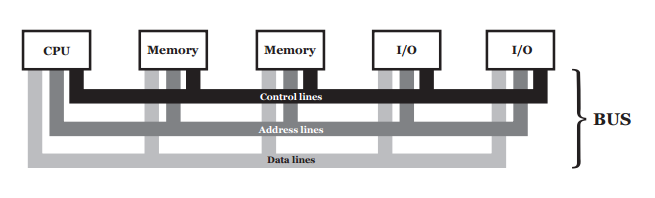
\includegraphics[width=15cm, keepaspectratio=yes]{imagenes/bus_sis.png}
\end{center}

Las líneas de datos y las de direcciones sirven para transmitir datos y direcciones, respectivamente. Las líneas de control se utilizan para transmitir tanto ordenes como información de temporización entre los módulos del sistema.

\subsection{Tipos de buses}
\subsubsection{Tipos de línea}
Pueden ser de dos tipos: Dedicadas ó Multiplexadas.
Las líneas dedicadas están permanentemente asignadas a una función (Dedicación funcional) o a un subconjunto físico de componentes del computador (Dedicación física).

\begin{center}
	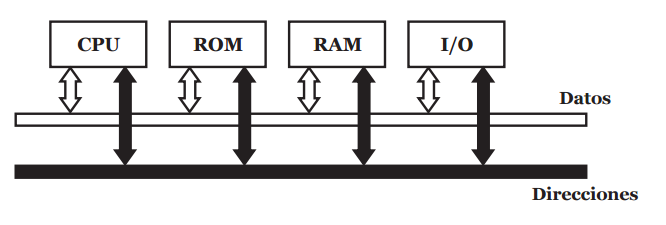
\includegraphics[width=10cm, keepaspectratio=yes]{imagenes/bus_dedicado.PNG}
\end{center}

Las líneas multiplexadas varían su propositos a lo largo del tiempo

\begin{center}
	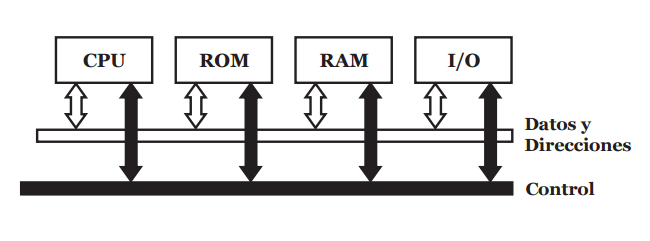
\includegraphics[width=10cm, keepaspectratio=yes]{imagenes/bus_multiplexado.PNG}
\end{center}

Aquí, la dirección se sitúa en el bus y se activa la línea de Dirección Válida. En ese momento, cada módulo dispone de un período de tiempo para copiar la dirección y determinar si es el módulo direccionado. Después, la dirección se quita del bus y las mismas conexiones se utilizan para la subsecuente transferencia de lectura o escritura de datos. Con este método se usan menos líneas por lo que se reducen espacio y costo. Sin embargo se necesita una circuitería mas compleja en cada modulo por lo que disminuye el rendimiento de la computadora.

\subsubsection{Ancho de bus}
La anchura del bus es la cantidad de líneas que tiene el mismo. Cuanto más ancho sea el bus de datos, es menor la cantidad de accesos a memoria ya que es mayor la cantidad de datos que se pueden transmitir simultáneamente.

La anchura del bus de direcciones afecta a la capacidad del sistema. Cuanto más ancho sea, mayor es el rango de posiciones a las que se puede hacer referencia.

\subsubsection{Temporización}
Los buses utilizan temporización síncrona o asíncrona para controlar la duración de los eventos.
Con temporización síncrona, la presencia de un evento en el bus está determinada por un reloj. El bus incluye una línea \textit{clk} a través de la cual transmite una secuencia en la que se alternan intervalos de igual duración de unos y ceros. Todos los eventos comienzan al principio de uno de estos ciclos (Un intervalo de unos más un intervalo de ceros).

Con la temporización asíncrona, la presencia de un evento en el bus es consecuencia de un evento previo. Este tipo de temporizadores es más difícil de implementar pero mejora el rendimiento de sistema cuando hay dispositivos con una gran diferencia de velocidades. La temporización síncrona, es mas fácil de implementar, pero las velocidades del reloj se deben adaptar a la velocidad del dispositivo más lento del sistema.

En un bus dedicado sincrónico, las transferencias ocupan un solo ciclo de reloj. En un multiplexado, toma 2 o más pues en el primer ciclo se manda la dirección a la cual se quiere escribir o de la cual se quiere leer y en los próximos ciclos se realiza la transferencia de datos.

\subsubsection{Arbitraje}
En todos los sistemas, más de un modulo puede necesitar el control del bus. Puesto que en un instante dado solo una unidad puede usar el bus, se requiere algún método de arbitraje. Este arbitraje puede ser centralizado o distribuido.

En un esquema centralizado, un dispositivo denominado \textbf{Bus Arbiter} es el responsable de asignar tiempo al bus

\begin{center}
	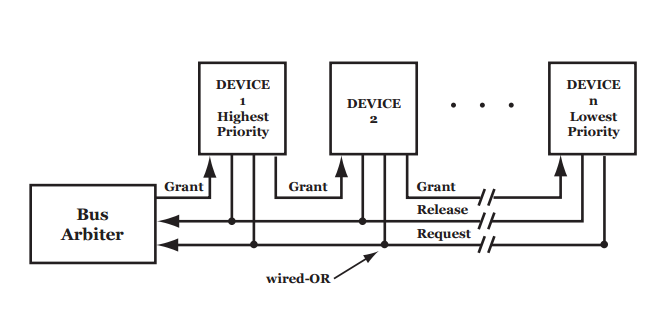
\includegraphics[width=10cm, keepaspectratio=yes]{imagenes/bus_arbitro.PNG}
\end{center}

En un esquema dsitribuido no existe dicho controlado. En su lugar, los módulos actuan conjuntamente para compartir el bus.

\begin{center}
	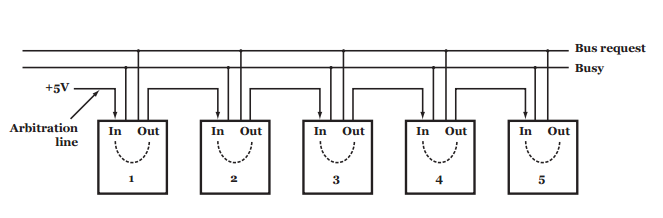
\includegraphics[width=10cm, keepaspectratio=yes]{imagenes/bus_no_arbitro.PNG}
\end{center}

\newpage

\section{Memoria}
Las memorias son los dispositivos utilizados para almacenar información y su rendimiento se mide según su:
\begin{itemize}
	\item Capacidad de almacenamiento
	\item Tiempo de acceso
	\item Velocidad de transferencia
	\item Consumo de energía
	\item Tamaño físico
	\item Costo total y costo por unidad de almacenamiento.
\end{itemize}

Como regla general, mientras más rápida sea la memoria, más alto es el costo por unidad de almacenamiento. Por lo que un computador podría llegar a ser muy caro si solo se usa memoria rápida o muy ineficiente si solo se usa memoria barata.

Para resolver este problema, y lograr un balance costo-beneficio adecuado, los computadores actuales usan un sistema jerárquico de memorias con diferentes velocidades y capacidades de almacenamiento clasificando a las memorias segun su ''distancia'' al CPU. Está jerarquía se muestra abajo en forma de pirámide.

\begin{center}
	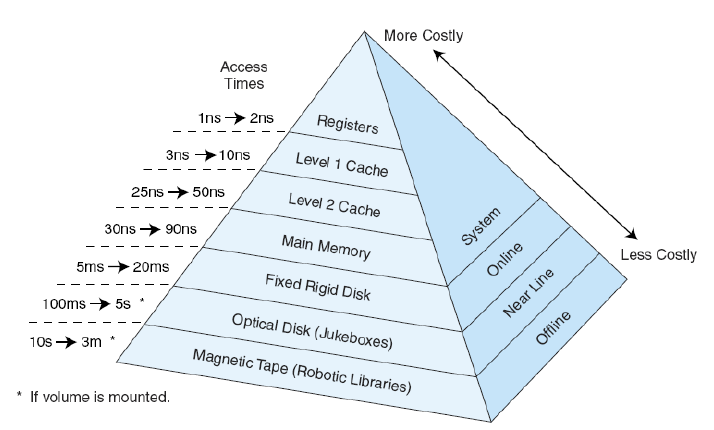
\includegraphics[width=10cm, keepaspectratio=yes]{imagenes/piramide.PNG}
\end{center}

Mientras más arriba de la pirámide, la memoria es más costosa, más rápida y más cercana al CPU se encuentra, pero es usada en menor cantidad. Cuando el CPU necesita información, la busca, primero, en el nivel más alto de la piramide. Sino lo encuentra, lo busca en el siguiente nivel.

Cuando el procesador encuentra los datos que necesita, copia el bloque de memoria que contiene dicho datos en un nivel de memoria superior para tener un acceso más rápido hacia el mismo. Esto se debe a que se busca acceder a la mayor cantidad de información posible de la manera más rápida y es muy probable que si se accedió a un dato de dicho bloque, se acceda a alguno de los datos subsecuentes.

Los distintos tipos de memorias usadas son:
\begin{itemize}
	\item \textbf{RAM (Random Access Memory)}: Memorias de lectura/escritura usada para almacenar programas y datos necesarios para la ejecución de un programa. Éstas memorias son volátiles, es decir que, cuando se les corta el suministro de energía, pierden toda la información almacenada en ellas.
	Hay dos tipos de memorias RAM: Dinámicas (\textbf{DRAM}) y Estáticas (\textbf{SRAM}). Las primeras requieren una recarga de energía cada pocos milisegundos para mantener la información, las SRAM mantienen la información mientras se le suministre energía, son más rápidas pero, también, más caras que las DRAM.
	
	Por lo general, las caché son bancos de memorias SRAM, mientras que la memoria principal es una DRAM.
	
	\item \textbf{ROM (Read-Only Memory)}: Memorias no volátiles que no pueden ser modificadas y son usadas en pequeñas cantidades para guardar información crítica del sistema, como pueden ser, las instrucciones de inicio. Este tipo de memoria tiene sus variantes que son las \textbf{PROM},\textbf{EPROM},\textbf{EEPROM} y las memorias \textbf{Flash} que son memorias ROM con las ventajas de que, a través de ciertos métodos, pueden ser borradas y reusadas.
	
\end{itemize}

\newpage

\section{Caché}
La memoria caché es un banco de memoria SRAM de muy alta velocidad que contiene una copia de los datos e instrucciones que están en la memoria principal. Su propósito es acelerar el acceso a estos ítem y así evitar \textit{wait states}.

Su tamaño debe ser lo suficientemente grande como para que el procesador pueda resolver la mayor cantidad posible de búsquedas de código y datos y lo suficientemente chica para no afectar el rendimiento ni el consumo de energía del sistema.

Cuando se realiza una búsqueda en la caché hay dos posibles resultados:
\begin{itemize}
	\item\textbf{Hit}: El ítem se encuentra en la caché
	\item\textbf{Miss}: El ítem no se encontró en la caché y tiene que ser buscado en la memoria principal.
\end{itemize}

Se define \textbf{HitRate} como la cantidad de hits sobre la cantidad de accesos a la caché:

$$hitRate = \frac{\#Hits}{\#Accesos~a~cache}$$

Y se considera que mientras mas alto sea el HitRate, mejor performance tiene la caché.

El siguiente diagrama muestra como se realizaria una operación de lectura de datos:

\begin{center}
	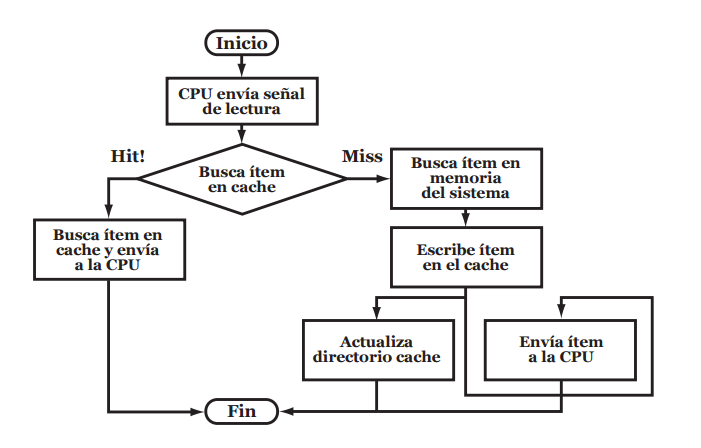
\includegraphics[width=10cm, keepaspectratio=yes]{imagenes/cache.PNG}
\end{center}


Para implementar este funcionamiento se necesita de un dispositivo especial llamado controlador de caché.

Al momento de copiar datos en la caché, el controlador actúa de acuerdo a dos principios que surgen de analizar el comportamiento de los algoritmos de software usados habitualmente:
\begin{itemize}
	\item\textbf{Principio de vecindad temporal}: Si un item es referenciado, la probabilidad de ser referenciado en el futuro inmediato es alta.
	\item\textbf{Principio de vecindad espacial}: Si un item es referenciado, es altamente probable que se referencien los vecinos a éste.
\end{itemize}
\subsection{Estructura de la caché}
Las cachés están divididas en líneas, que son el elemento mínimo de palabra de datos dentro de la caché. El tamaño de las líneas corresponde a un múltiplo de la palabra de datos de memoria. Esto se debe a que cuando se direcciona un ítem en memoria, se requerirá de los ítem que lo rodean.

Para guardar estos datos, el controlador de la caché debe saber en que lugar ubicarlo para obtener un acceso rápido. Para esto, cuando el procesador le pasa una dirección de memoria, éste agrupa sus bits en tres conjuntos:
\begin{itemize}
	\item\textbf{Tag}: Identifica el número del bloque al que pertenece la línea en la memoria principal.
	\item\textbf{Línea o Set}: Indica en qué posición de la caché se ubica la línea.
	\item\textbf{Índice}: Indica en qué posición de la línea se encuentra el dato pedido.
\end{itemize}
Una vez conseguidos estos conjuntos, el controlador ubica en la caché dicha línea respetando ciertas politicas de decisión. Algunas de estas políticas son:
\begin{itemize}
	\item\textbf{Mapeo Directo}: La línea se ubica en el número de línea indicado por \textit{set}
	\item\textbf{Asociativa de 2 vías}: En este caso, la caché es divida en 2 y se toma a cada mitad como una caché por separado. En este caso, \textit{set} indica a que mitad de la cache le corresponde almacenar la línea. Y la línea es almacenada en cualquier lugar disponible de esa mitad.
\end{itemize}

En el caso de que se use una caché asociativa, además, se debe elegir alguna política de desalojo de bloques, es decir, si la caché esta llena y se produce un miss, entonces habrá que remplazar alguna linea guardada por la nueva que se pide a la memoria principal. Estas políticas pueden ser:
\begin{itemize}
	\item\textbf{LRU} (Least Recently Used): Se borra el bloque que hace más tiempo que no es usado
	\item\textbf{LFU} (Least Frequently Used): Se borra el bloque que menos haya sido usado.
	\item\textbf{FIFO} (First In First Out): Se borra el bloque que hace más tiempo que está en la cache.
\end{itemize}

\subsection{Impacto del caché miss}
En los computadores actuales, el pipeline es un mecanismo que permite superponer, en el tiempo, la ejecución de varias instrucciones a la vez. Si la búsqueda de una instrucción o un operando falla, entonces el procesador debe recurrir a la memoria principal. La demora en este acceso hace que el pipeline se atasque y se ocupen varios ciclos de reloj para que vuelva a tomar su ritmo de ejecución normal.

\subsection{Escritura de datos}
Llegado el momento, el procesador querrá modificar algún dato de la memoria, si esto sucede se debe asegurar que este cambio se vea reflejado tanto en la caché como en la memoria principal. Para lograr esto se puede usar algunos de los siguientes mecanismos:
\begin{itemize}
	\item\textbf{Write Through}: El procesador escribe la DRAM y el controlador caché refresca la caché con el dato actualizado.
	\item\textbf{Write Through Buffered}: El procesador actualiza la caché y el controlador caché, luego, actualiza la DRAM mientras el procesador sigue ejecutando instrucciones y usando datos de la memoria caché
	\item\textbf{Copy Back}: Se marcan las líneas de la memoria caché cuando el procesador escribe en ellas. Luego, en el momento de eliminar esas líneas del caché, el controlador deberá actualizar la copia en la DRAM.
\end{itemize}

En todos los casos, si se produce un miss mientras el controlador caché esta actualizando las copias, el procesador debe esperar a que se termine este proceso.
\nocite{*}
\bibliographystyle{plain}
\bibliography{bibliography}
\end{document}

